% Copyright (C) 2013 - Michael Baudin
%
% This file must be used under the terms of the 
% Creative Commons Attribution-ShareAlike 3.0 Unported License :
% http://creativecommons.org/licenses/by-sa/3.0/

\chapter{Projections}

The goal of this page is to gather experiments showing bad 2D projections
for low disrepancy sequences. 
%%%%%%%%%%%%%%%%%%%%%%%%%%%%%%%%%%%%%%%%%%%%%%%%%%%%%%%%%%%%%%%%%%


  
\section{Halton Sequence}

In this section, we present some bad 2D projections of the Halton sequence.
The Halton sequence is known for having bad 2D projections and
several examples are presented in the bibliography.

In the following example, we consider the projection of dimensions (28,29)
as in \cite{Chi:2005:OHS:1744084.1744136}. 
The paper contains an error : the faulty projection is
(28,29) (primes 107,109) and not (27,28) (primes 103,107). 
We use the \scifun{corrcoef} function from the Stixbox module, 
which computes the correlation coefficient between two samples.

\lstset{language=scilabscript}
\begin{lstlisting}
u=lowdisc_ldgen ( 4096 , 29 , "halton" );
scf(); 
lowdisc_proj2d ( u , [28 29] );
// Compute the correlation coefficient for dimensions (28,29)
corrcoef ( [u(:,28) u(:,29)] )
\end{lstlisting}

The previous script produces the following output.

\lstset{language=scilabscript}
\begin{lstlisting}
-->corrcoef ( [u(:,28) u(:,29)] )
 ans  =
    1.         - 0.1210675  
  - 0.1210675    1.         
\end{lstlisting}

The previous script also produces the figure \ref{fig-halton-proj28-29}.

\begin{figure}[htbp]
\begin{center}
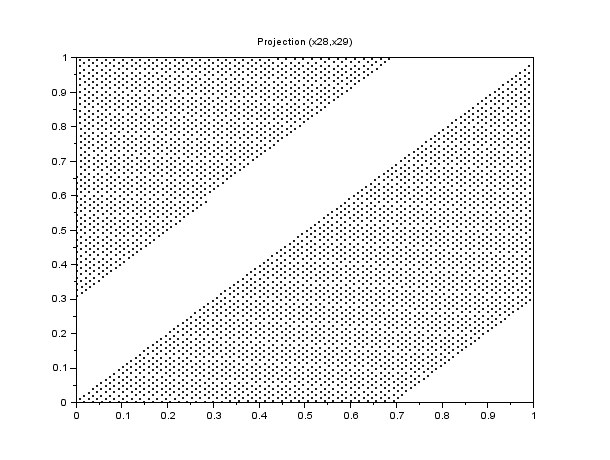
\includegraphics[width=15cm]{figures/halton-proj28-29.png}
\end{center}
\caption{The Halton sequence - 4096 points in 29 dimensions. Projection (28,29).}
\label{fig-halton-proj28-29}
\end{figure}

The figure \ref{fig-halton-proj28-29-leaped} presents the leaped - Halton sequence. 
There is no obvious problem anymore.

\lstset{language=scilabscript}
\begin{lstlisting}
u=lowdisc_ldgen ( 4096 , 29 , "halton-leaped");
scf(); 
lowdisc_proj2d ( u , [28 29] );
\end{lstlisting}

\begin{figure}[htbp]
\begin{center}
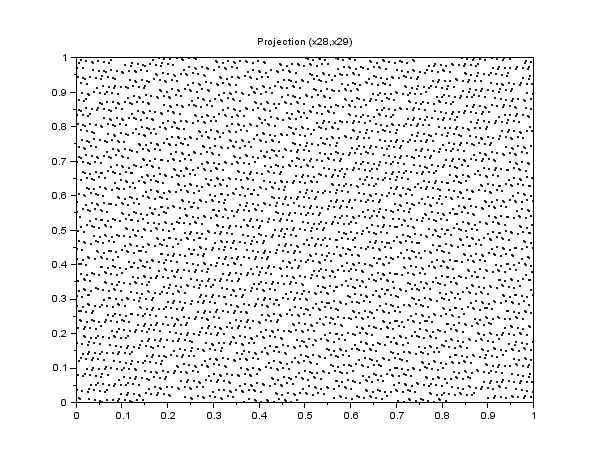
\includegraphics[width=15cm]{figures/halton-proj28-29-leaped.png}
\end{center}
\caption{The leaped Halton sequence - 4096 points in 29 dimensions. Projection (28,29).}
\label{fig-halton-proj28-29-leaped}
\end{figure}

In the following example, we consider the projection of Halton
sequence in dimensions (39,40)
as suggested by Kocis and Whiten \cite{Kocis1997}.

\lstset{language=scilabscript}
\begin{lstlisting}
u=lowdisc_ldgen ( 2000 , 40 , "halton" );
scf();
lowdisc_proj2d ( u , [39 40] );
// Compute the correlation coefficient for dimensions (39,40)
corrcoef ( [u(:,39) u(:,40)] )
\end{lstlisting}

The previous script produces the following output.

\lstset{language=scilabscript}
\begin{lstlisting}
-->corrcoef ( [u(:,39) u(:,40)] )
 ans  =
    1.           0.1048947  
    0.1048947    1.         
\end{lstlisting}


The previous script also produces the figure \ref{fig-halton-proj39-40}.

\begin{figure}[htbp]
\begin{center}
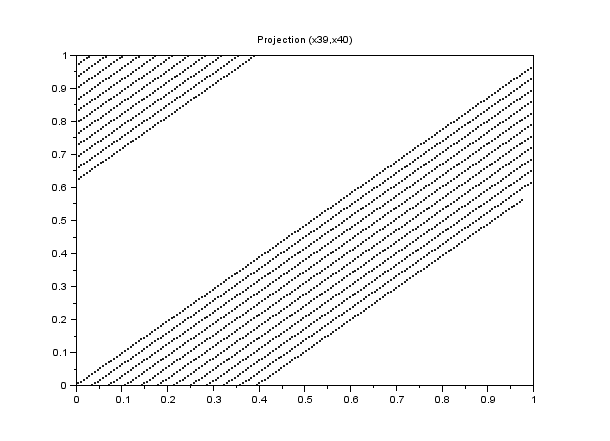
\includegraphics[width=15cm]{figures/halton-proj39-40.png}
\end{center}
\caption{The Halton sequence - 2000 points in 40 dimensions. Projection (39,40).}
\label{fig-halton-proj39-40}
\end{figure}

The following script performs the same experiment with the 
leaped-Halton.

\lstset{language=scilabscript}
\begin{lstlisting}
u=lowdisc_ldgen ( 2000 , 40 , "halton-leaped");
scf();
lowdisc_proj2d ( u , [39 40] );

\end{lstlisting}

The previous script produces the figure \ref{fig-halton-proj39-40-leaped}.

\begin{figure}[htbp]
\begin{center}
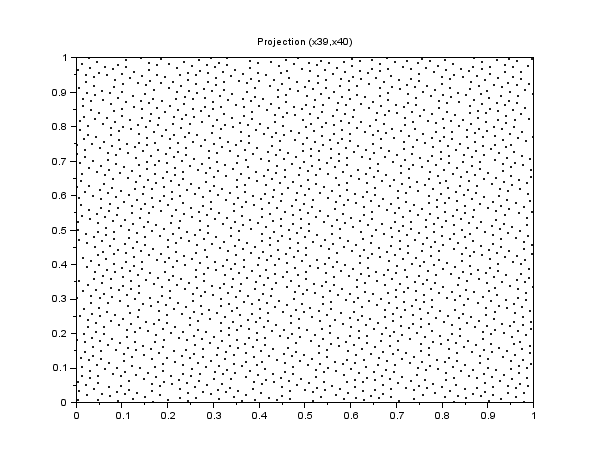
\includegraphics[width=15cm]{figures/halton-proj39-40-leaped.png}
\end{center}
\caption{The leaped Halton sequence - 2000 points in 40 dimensions. Projection (39,40).}
\label{fig-halton-proj39-40-leaped}
\end{figure}
    
On the other hand, we emphasize that a leaped Faure sequence is 
not a (0,s)-sequence anymore. 
Therefore, there is no guarantee that the leaped Faure sequence is 
a low discrepancy sequence.

In the following example, we search the worst Halton projection
for 2000 points in dimensions 40.
In order to evaluate the projection, we compute the
correlation coefficients.
The projections which have the largest non-diagonal
correlation coefficients are the worst.

\lstset{language=scilabscript}
\begin{lstlisting}
u=lowdisc_ldgen ( 2000 , 40 , "halton" );
// Compute correlation coefficients
c = corrcoef ( u );
// Get the maximum correlation coefficient 
// but remove the diagonal (unity) terms
[m,k] = max(abs(c-eye(c)))
// This is projection (35,36) :
k
// Get the correlation coefficient for this projection
c(k(1),k(2))
// Print this projection
scf();
lowdisc_proj2d ( u , k );
\end{lstlisting}

The previous script produces the figure \ref{fig-halton-proj35-36}.

\begin{figure}[htbp]
\begin{center}
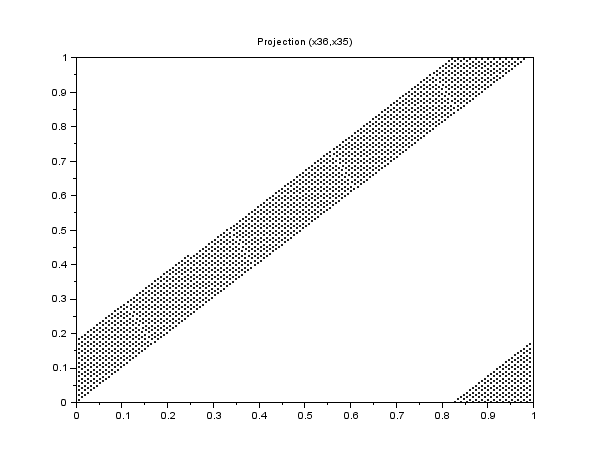
\includegraphics[width=15cm]{figures/halton-proj35-36.png}
\end{center}
\caption{The Halton sequence - 2000 points in 40 dimensions. Projection (35,36).}
\label{fig-halton-proj35-36}
\end{figure}
    

%%%%%%%%%%%%%%%%%%%%%%%%%%%%%%%%%%%%%%%%%%%%%%%%%%%%%%%%%%%%%%%%%%

\section{Faure Sequence}

In this section, we present some bad 2D projections of the Faure sequence.

In the following example, we search for the worst
projection of 2000 points of the Faure sequence in dimension 40.
The worst projection is relatively good, which
indicates how Faure's sequence is much better than Halton's sequence.

\lstset{language=scilabscript}
\begin{lstlisting}
u=lowdisc_ldgen ( 2000 , 40 , "faure" );
// Compute correlation coefficients
c = corrcoef ( u );
// Get the maximum correlation coefficient 
// but remove the diagonal (unity) terms
[m,k] = max(abs(c-eye(c)))
// This is projection (20,21) :
k
// Get the correlation coefficient for this projection
c(k(1),k(2))
// Print this projection
scf();
lowdisc_proj2d ( u , k );
\end{lstlisting}

The previous script produces the figure \ref{fig-faure-proj21-20}.
    
\begin{figure}[htbp]
\begin{center}
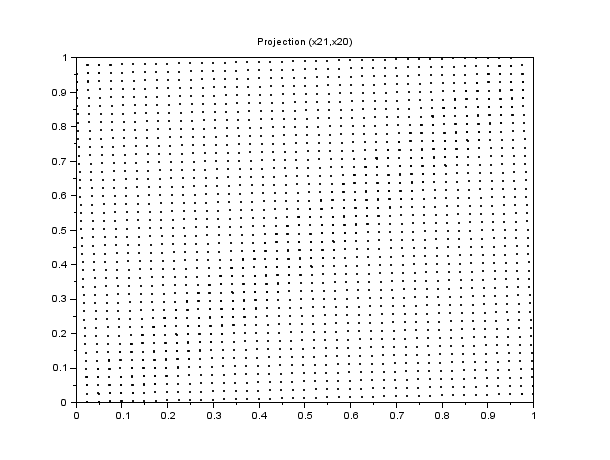
\includegraphics[width=15cm]{figures/faure-proj21-20.png}
\end{center}
\caption{The Faure sequence - 2000 points in 40 dimensions. Projection (20,21).}
\label{fig-faure-proj21-20}
\end{figure}

This is consistent with the fact that, in s=40 dimensions,
the Faure sequence uses the prime number b=41 as the base.
Moreover, the Faure sequence in dimension s=40 is
a (0,40)-sequence in base b=41.
Consider now the projection (i,j), for i different from j. 
Consider elementary intervals from 41 subdivisions
in dimension i, 41 subdivisions in dimension j, and 
1 subdivision in the other dimensions.
There are $41^2=1681$ intervals, each with volume 1/1681. 
Hence, if we consider a set of 1681 points, each such constructed 
elementary interval has one point. 
Since the previous figure has 2000>1681 points, all 2D projections 
of the Faure sequence in dimension s=40 are quite well distributed.

In the following example, we consider 300 points of the Faure
sequence in dimension 40, and consider the projection (39,40)
as suggested by Kocis and Whiten \cite{Kocis1997}.

\lstset{language=scilabscript}
\begin{lstlisting}
u=lowdisc_ldgen ( 300 , 40 , "faure" );
scf();
lowdisc_proj2d ( u , [39 40] );
\end{lstlisting}

The previous script produce the figure \ref{fig-faure-proj39-40}.

\begin{figure}[htbp]
\begin{center}
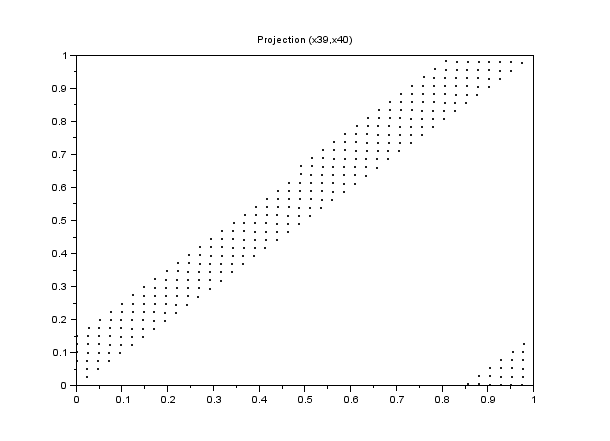
\includegraphics[width=15cm]{figures/faure-proj39-40.png}
\end{center}
\caption{The Faure sequence - 300 points in 40 dimensions. Projection (39,40).}
\label{fig-faure-proj39-40}
\end{figure}

Since the number of points is 300 which is much smaller than $41^2=1681$, 
the Faure sequence cannot evenly distribute the points in the space. 

We check what is the behavior with more favorable parameters. 

\lstset{language=scilabscript}
\begin{lstlisting}
dim = 40;
nsimmin = 300;
lds = lowdisc_new("faure");
lds = lowdisc_configure(lds,"-dimension",dim);
base = lowdisc_get(lds,"-faureprime");
[nsim,skip,leap] = lowdisc_fauresuggest ( dim , base , nsimmin );
lds = lowdisc_configure(lds,"-skip",skip);
lds = lowdisc_configure(lds,"-leap",leap);
[lds,u]=lowdisc_next(lds,nsim);
lds = lowdisc_destroy(lds);
scf();
lowdisc_proj2d ( u , [39 40] );
\end{lstlisting}

We see that the number of experiments has increased from 300
to 68921, which is significantly more. 

\lstset{language=scilabscript}
\begin{lstlisting}
-->size(u)
 ans  =
    68921.    40.  
  \end{lstlisting}

The figure \ref{fig-faure-n68921-proj39-40} shows that there the correlation problem 
is greatly reduced, although the points seems to be located 
on lines.

\begin{figure}[htbp]
\begin{center}
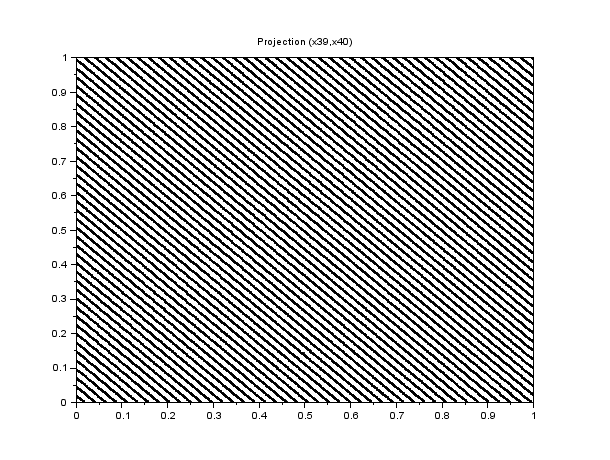
\includegraphics[width=15cm]{figures/faure-n68921-proj39-40.png}
\end{center}
\caption{The Faure sequence - 68921 points in 40 dimensions. Projection (39,40).}
\label{fig-faure-n68921-proj39-40}
\end{figure}

The number of points $68921=41^3$, which guarantees good 3D projections. 

In order to keep the number of experiments constant, we might be 
interested in using the \scivar{leap} option.
Following Kocis and Whithen \cite{Kocis1997}, 
we may try a leaped Faure sequence. 
We try the leap L=5.

\lstset{language=scilabscript}
\begin{lstlisting}
lds = lowdisc_new("faure");
lds = lowdisc_configure(lds,"-dimension",40);
lds = lowdisc_configure(lds,"-leap",5);
[lds,u] = lowdisc_next (lds,300);
lds = lowdisc_destroy(lds);
scf();
lowdisc_proj2d ( u , [39 40] );
\end{lstlisting}

The previous script produces the figure \ref{fig-faure-n300-leaped-proj39-40}.

\begin{figure}[htbp]
\begin{center}
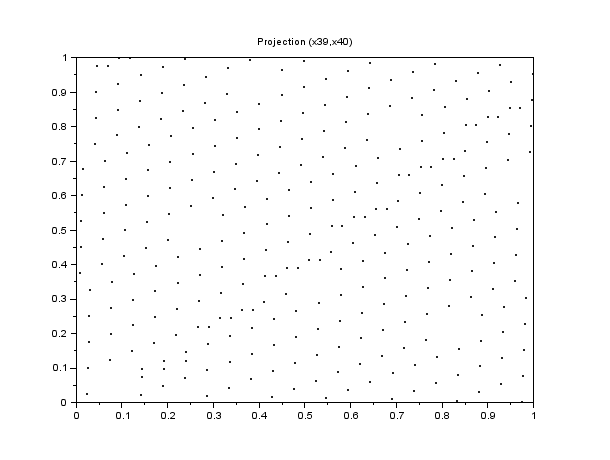
\includegraphics[width=15cm]{figures/faure-n300-leaped-proj39-40.png}
\end{center}
\caption{The Faure sequence - 300 points in 40 dimensions. Projection (39,40).}
\label{fig-faure-n300-leaped-proj39-40}
\end{figure}
    
On the other hand, we emphasize that a leaped Faure sequence is 
not a (0,s)-sequence anymore. 
Therefore, there is no guarantee that the leaped Faure sequence is 
a low discrepancy sequence.

%%%%%%%%%%%%%%%%%%%%%%%%%%%%%%%%%%%%%%%%%%%%%%%%%%%%%%%%%%%%%%%%%%

\section{Sobol Sequence}

In this section, we present some bad 2D projections of the Sobol sequence.

In the following example, we consider 1000 points of the  
Sobol sequence in 23 dimensions and check the 
projection (16,23).

\lstset{language=scilabscript}
\begin{lstlisting}
u=lowdisc_ldgen(1000,30,"sobol");
scf();
lowdisc_proj2d(u,[16 23])
xtitle("Sobol : 1000 points","X16","X23")
\end{lstlisting}

The previous script produces the figure \ref{fig-sobol-s23-proj16-23}.

\begin{figure}[htbp]
\begin{center}
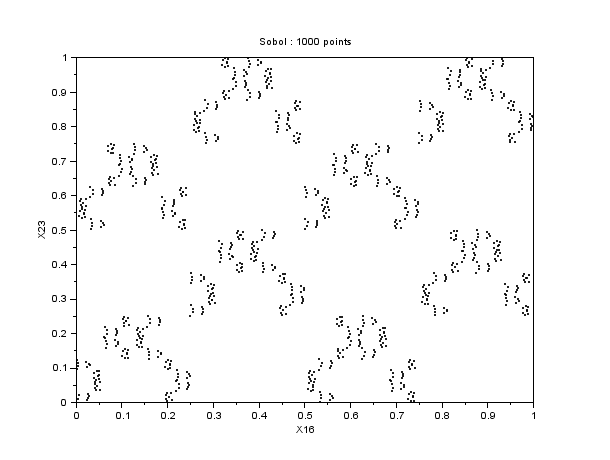
\includegraphics[width=15cm]{figures/sobol-s23-proj16-23.png}
\end{center}
\caption{The Sobol sequence - 1000 points in 30 dimensions. Projection (16,23).}
\label{fig-sobol-s23-proj16-23}
\end{figure}

In the following example, we consider 
1000 points of the Sobol sequence in 36 dimensions and 
check the projection (11,36).

\lstset{language=scilabscript}
\begin{lstlisting}
u=lowdisc_ldgen(1000,36,"sobol");
scf();
lowdisc_proj2d(u,[11 36])
xtitle("Sobol : 1000 points","X11","X36")
\end{lstlisting}

The previous script produces the figure \ref{fig-sobol-s36-proj11-36}.

\begin{figure}[htbp]
\begin{center}
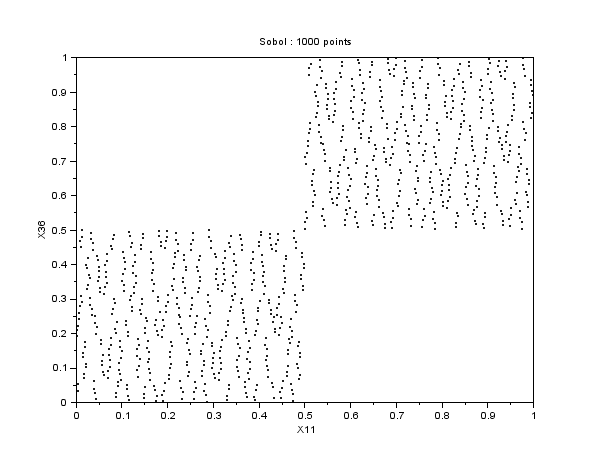
\includegraphics[width=15cm]{figures/sobol-s36-proj11-36.png}
\end{center}
\caption{The Sobol sequence - 1000 points in 36 dimensions. Projection (11,36).}
\label{fig-sobol-s36-proj11-36}
\end{figure}

In the following example, we plot the projection 
(5,22) of $2^{12}$ and $2^{13}$ 
points of the Sobol sequence in s=22 dimensions. 
This example is presented in \cite{Joe:2008:CSS:1405171.1405191}. 
We consider $2^{m-t}=2^4 \times 2^2=2^6$ elementary intervals, 
with $2^4$ divisions in the dimension $x_5$ 
and $2^2$ divisions in the dimension $x_{22}$. 
For this projection, the quality parameter t is 7. 
Hence, we need $2^m=2^{6+7}=2^{13}$ points 
to make so that each elementary interval contain 
$2^t=2^7$ points.

\lstset{language=scilabscript}
\begin{lstlisting}
h=scf();
subplot(2,1,1);
//
b=2;
s=22;
m=12;
r = [4 2];
N=b^m;
u=lowdisc_ldgen(N-1,s,"sobol");
u=[zeros(1,s);u];
plot(u(:,5),u(:,22),"b.")
lowdisc_plotelembox([b b],r)
xtitle(msprintf("Volume=1/%d, %d Points",..
  b^sum(r),N),"X5","X22")
//
subplot(2,1,2);
m=13;
N=b^m;
u=lowdisc_ldgen(N-1,s,"sobol");
u=[zeros(1,s);u];
plot(u(:,5),u(:,22),"b.")
lowdisc_plotelembox([b b],r)
xtitle(msprintf("Volume=1/%d, %d Points",..
  b^sum(r),N),"X5","X22")
//
h.children(1).isoview="off";
h.children(2).isoview="off";
h.children(1).children($).children.mark_size=2;
h.children(2).children($).children.mark_size=2;
\end{lstlisting}

The previous script produces the figure \ref{fig-sobol-s22-proj5-22}.

\begin{figure}[htbp]
\begin{center}
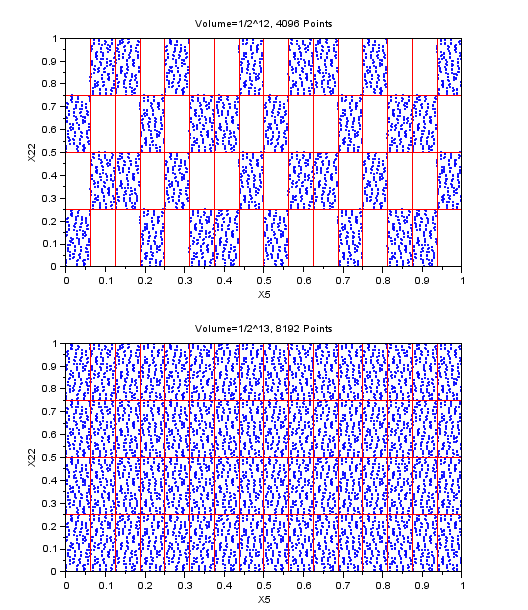
\includegraphics[width=15cm]{figures/sobol-s22-proj5-22.png}
\end{center}
\caption{The Sobol sequence - $2^{12}$ (top) and $2^{13}$ (bottom) points in 22 dimensions. Projection (5,22).}
\label{fig-sobol-s22-proj5-22}
\end{figure}

%%%%%%%%%%%%%%%%%%%%%%%%%%%%%%%%%%%%%%%%%%%%%%%%%%%%%%%%%%%%%%%%%%

\section{Niederreiter (base 2) Sequence}
\label{sec-projnieder}

In this section, we consider 1000 points of the 
Niederreiter (base 2) sequence in 26 dimensions, 
and consider the projection (25,26).

\lstset{language=scilabscript}
\begin{lstlisting}
u=lowdisc_ldgen(1000,30,"niederreiter");
scf();
lowdisc_proj2d(u,[25 26])
\end{lstlisting}

The previous script produce the figure \ref{fig-niederreiter-s26-n1000}.

\begin{figure}[htbp]
\begin{center}
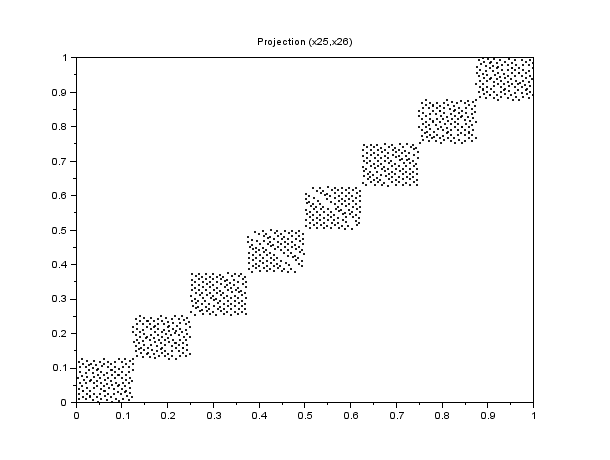
\includegraphics[width=15cm]{figures/niederreiter-s26-n1000.png}
\end{center}
\caption{The Niederreiter (base 2) sequence - 1000 points in 30 dimensions. Projection (25,26).}
\label{fig-niederreiter-s26-n1000}
\end{figure}
  
%%%%%%%%%%%%%%%%%%%%%%%%%%%%%%%%%%%%%%%%%%%%%%%%%%%%%%%%%%%%%%%%%%

\section{Two-dimensional correlations with increasing dimensions}

In this section, we present how the linear correlation 
coefficient between dimensions of the sequence deteriorates 
when the number of dimensions increases. 
Given a number of dimensions and 1000 points, we are 
interested in the worst 2D projection, as defined by 
the largest correlation coefficient.


%%%%%%%%%%%%%%%%%%%%%%%%%%%%%%%%%%%%%%%%%%%%%%%%%%%%%%%%%%%%%%%%%%
\subsection{Numerical experiments}

The following function test for low discrepancy sequences for 
dimensions s from 2 to smax. 
It generates a low discrepancy point set for n points and computes 
the correlation coefficient between columns of the matrix. 
Then the diagonal terms are set to zero and the largest entry is computed. 
We assume here that this identifies the worst 2D projection. 

\lstset{language=scilabscript}
\begin{lstlisting}
function m=worstCorrelation(n,smax,seqname)
    for s=2:smax
        u=lowdisc_ldgen(n,s,seqname);
        c = corrcoef ( u );
        m(s-1) = max(abs(c-eye(c)));
    end
endfunction
\end{lstlisting}

The following script tests the Halton, Sobol, Faure and Niederreiter (optimal base) 
sequences.

\lstset{language=scilabscript}
\begin{lstlisting}
n=1000;
smax=50;
scf();
m=worstCorrelation(n,smax,"halton");
plot(2:smax,m,"r-")
m=worstCorrelation(n,smax,"sobol");
plot(2:smax,m,"b-")
m=worstCorrelation(n,smax,"faure");
plot(2:smax,m,"g-")
m=worstCorrelation(n,smax,"niederreiter");
plot(2:smax,m,"k-")
legend(["Halton","Sobol","Faure",..
"Niederreiter"]);
a=gca();
a.children(1).legend_location="in_upper_left";
xtitle("1000 Points","Number of dimensions",..
"Maximum Correlation Coefficient")
  \end{lstlisting}

The previous script produces figure \ref{fig-badcorr1}.
This shows that, according to this test, the Niederreiter 
sequence in base 2 performs well for $s<15$, but 
rapidely deteriorates for $s\geq15$. 
Notice that that optimal base of Niederreiter sequence is known 
by our implementation only for $s<13$. 
As expected, the Halton sequence has poor 2D projections, 
especially for $s\geq 20$ where the correlation coefficient 
becomes larger than 0.1. 
The Sobol sequence is better than Halton, but can have poor 2D projections, 
especially for $s\geq 35$. 
However, the projections for $s<25$ are the best of this test. 
The Faure sequence appears to be the most robust sequence in this 
test for high dimensions.

\begin{figure}[htbp]
\begin{center}
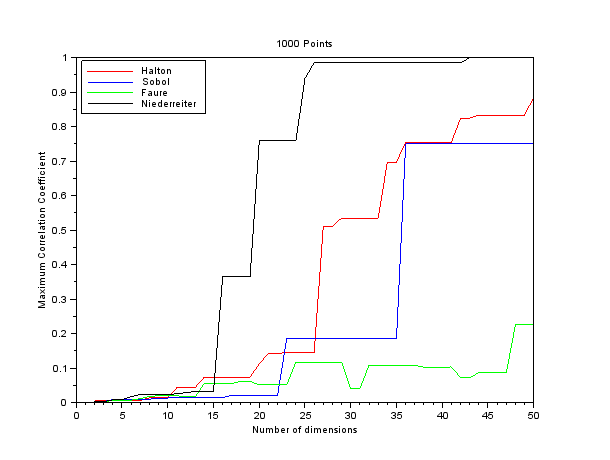
\includegraphics[width=15cm]{figures/badcorr1.png}
\end{center}
\caption{The maximum correlation coefficient vs the number of dimensions for various low 
discrepancy sequences.}
\label{fig-badcorr1}
\end{figure}

The following script tests various Halton 
sequences.

\lstset{language=scilabscript}
\begin{lstlisting}
n=1000;
smax=50;
scf();
m=worstCorrelation(n,smax,"halton");
plot(2:smax,m,"r-")
m=worstCorrelation(n,smax,"sobol");
plot(2:smax,m,"b-")
m=worstCorrelation(n,smax,"faure");
plot(2:smax,m,"g-")
m=worstCorrelation(n,smax,"niederreiter");
plot(2:smax,m,"k-")
legend(["Halton","Sobol","Faure",..
"Niederreiter"]);
a=gca();
a.children(1).legend_location="in_upper_left";
xtitle("1000 Points","Number of dimensions",..
"Maximum Correlation Coefficient")
  \end{lstlisting}

The previous script produces figure \ref{fig-badcorr2}.
This shows that, according to this test, the reverse Halton 
sequence has almost the same poor 2D projections as the Halton 
sequences (the two red lines are almost the same). 
The leaped Halton sequence generally has better projections than Halton, 
but can also have larger correlations (s=16, 24, 42). 
The scrambled (Kocis-Whiten) Halton sequence is the most robust 
sequence in this test, at the exception of s=25, for which 
the correlation is slightly larger. 
These graphics suggest that the scrambled Halton sequence is the best of 
this set of tests.

\begin{figure}[htbp]
\begin{center}
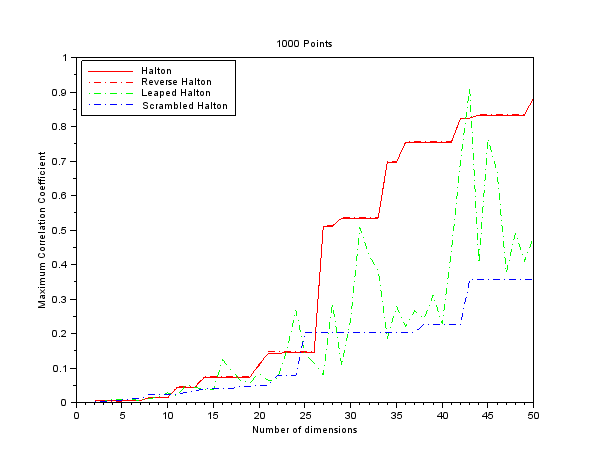
\includegraphics[width=15cm]{figures/badcorr2.png}
\end{center}
\caption{The maximum correlation coefficient vs the number of dimensions for various low 
discrepancy sequences.}
\label{fig-badcorr2}
\end{figure}

%%%%%%%%%%%%%%%%%%%%%%%%%%%%%%%%%%%%%%%%%%%%%%%%%%%%%%%%%%%%%%%%%%
\subsection{Conclusions}

These tests suggest that the Sobol sequence is better 
for small dimensions ($s<25$) and the Faure sequence 
is better for large dimensions ($s>25$). 
Weirdly, the Niederreiter sequence performs poorly in this test. 
However, this confirms the poor projections we have presented in the 
section \ref{sec-projnieder}.

We do not see any practical difference between the Reverse Halton 
sequence and the Halton sequence in terms of 2D projections. 
the scrambled 
On the other hand, the scrambled Halton sequence is generally better than a classical Halton 
sequence.
